\documentclass[aspectratio=169]{beamer}

% ---------------------------------------------------------------------------
% NYU-violet themed deck for Hybrid-NL2SVA.
%   Part I  -- the Hybrid-NL2SVA pipeline itself + cross-model FVEval-Verified
%              comparison results.
%   Part II -- end-to-end Spec2SVA: AssertionForge (Stage 1+2 = Spec2NL)
%              feeding Hybrid-NL2SVA (NL2SVA), UART pilot.
% ---------------------------------------------------------------------------

\usepackage{fontspec}
\usepackage{graphicx}
\usepackage{tikz}
\usetikzlibrary{arrows.meta, positioning, fit, backgrounds, shapes.geometric}
\usepackage{booktabs}
\usepackage{array}
\usepackage{multirow}
\usepackage{xcolor}
\usepackage{listings}

% ------------------------------ NYU palette ---------------------------------
% Light theme (2026-09-03 rework, replacing the earlier all-violet-canvas
% look): white content canvas, NYU violet reserved for accents/headings, a
% dark-violet "hero" treatment kept only for the title page and the Part
% divider frames (\dividerframe) for pacing/contrast -- a common academic-
% deck pattern (bold cover + section breaks, readable light content pages).
\definecolor{nyuviolet}{HTML}{57068C}      % NYU primary violet -- headings, accents
\definecolor{nyuvioletdark}{HTML}{3C0561}  % darker shade -- hero backgrounds, diagram fills/arrows
\definecolor{nyuvioletlight}{HTML}{B185D6} % pale violet -- soft rules/borders (legible on white OR dark)
\definecolor{nyumuted}{HTML}{7A5A99}       % muted violet -- secondary text on the WHITE canvas (subtitles, notes, footline)
\definecolor{nyulavender}{HTML}{F1E9FA}    % very pale panel background (light theme)
\definecolor{cardwhite}{HTML}{FFFFFF}
\definecolor{cardtext}{HTML}{221033}
\definecolor{bodytext}{HTML}{2B2438}       % near-black body text on white canvas
\definecolor{goodgreen}{HTML}{2E8B57}
\definecolor{warnamber}{HTML}{C97A1F}

\setbeamertemplate{navigation symbols}{}
\setbeamercolor{background canvas}{bg=white}
\setbeamercolor{normal text}{fg=bodytext}
\setbeamercolor{title}{fg=white}
\setbeamercolor{subtitle}{fg=nyuvioletlight}
\setbeamercolor{author}{fg=white}
\setbeamercolor{date}{fg=nyuvioletlight}
\setbeamercolor{frametitle}{fg=nyuviolet}
\setbeamercolor{framesubtitle}{fg=nyumuted}
\setbeamercolor{structure}{fg=nyuviolet}
\setbeamercolor{itemize item}{fg=nyuviolet}
\setbeamercolor{itemize subitem}{fg=nyuviolet}
\setbeamercolor{section in toc}{fg=bodytext}
\setbeamercolor{subsection in toc}{fg=nyumuted}
\setbeamercolor{page number in head/foot}{fg=nyumuted}
\setbeamertemplate{itemize item}{\raise1pt\hbox{\small\textbullet}}
\setbeamertemplate{itemize subitem}{\raise1pt\hbox{\footnotesize\textendash}}
\setbeamerfont{frametitle}{series=\bfseries, size=\Large}
\setbeamerfont{footline}{size=\tiny}

\setbeamertemplate{frametitle}{
  \vspace{4pt}
  {\usebeamerfont{frametitle}\usebeamercolor[fg]{frametitle}\insertframetitle}\\[-2pt]
  {\usebeamerfont{framesubtitle}\usebeamercolor[fg]{framesubtitle}\insertframesubtitle}
  \vspace{2pt}
  \hrule height 1pt \color{nyuvioletlight}
  \vspace{6pt}
}

\setbeamertemplate{footline}{
  \leavevmode
  \hbox{\begin{beamercolorbox}[wd=\paperwidth,ht=2.4ex,dp=1ex,left,leftskip=1em,right,rightskip=1em]{page number in head/foot}
    \textcolor{nyumuted}{\scriptsize Hybrid-NL2SVA}
    \hfill
    \textcolor{nyumuted}{\scriptsize\insertframenumber\,/\,\inserttotalframenumber}
  \end{beamercolorbox}}
}

% A "card": pale lavender rounded panel for data-heavy content (tables,
% code), grouping it visually against the white canvas.
\setbeamercolor{card}{bg=nyulavender, fg=cardtext}
\newenvironment{card}[1][\textwidth]{%
  \begin{beamercolorbox}[wd=#1,sep=8pt,rounded=true,shadow=false]{card}
}{%
  \end{beamercolorbox}
}

% Compact colored pill/tag, e.g. for status labels.
\newcommand{\statuspill}[2]{\tikz[baseline=-0.6ex]{\node[fill=#1, text=white, rounded corners=2pt, inner sep=3pt, font=\scriptsize\bfseries]{#2};}}

% A plain divider frame standing in for beamer's \part/\partpage -- real
% \part commands make bare \tableofcontents only show the CURRENT part's
% sections (empty when called before any \part begins, which is where an
% Outline slide belongs), so this sidesteps that entirely: no \part command,
% no beamer part-tracking, sections stay globally visible to \tableofcontents.
% Kept as a full-bleed dark-violet "hero" frame (matching the title page)
% for visual pacing against the light content frames elsewhere.
\newcommand{\dividerframe}[2]{%
  \begin{frame}[plain]
    \begin{tikzpicture}[remember picture, overlay]
      \fill[nyuviolet] (current page.south west) rectangle (current page.north east);
    \end{tikzpicture}
    \vfill
    \begin{center}
      {\Large\textcolor{nyuvioletlight}{Part #1}}\\[10pt]
      {\Huge\bfseries\textcolor{white}{#2}}
    \end{center}
    \vfill
  \end{frame}
}

\title{\textbf{Hybrid-NL2SVA}}
\subtitle{A RAG+Self-Correction Pipeline for NL2SVA, Cross-Model Evaluation,\\and an End-to-End Spec2SVA Extension via AssertionForge}
\author{Hybrid-NL2SVA Project}
\institute{New York University}
\date{\today}

\begin{document}

% ============================================================================
% Title page: light canvas (matching the rest of the deck), the real NYU
% wordmark (extracted 2026-09-03 from nyu.edu's own homepage header SVG,
% recolored from its native white-on-violet-header to NYU violet for use
% on our white canvas -- not a hand-drawn placeholder, not a third-party
% mirror) placed bottom-left, and a two-line Part I/II summary.
\begin{frame}[plain]
  \begin{tikzpicture}[remember picture, overlay]
    \node[anchor=south west, xshift=0.6cm, yshift=0.4cm] at (current page.south west) {
\includegraphics[width=1.3cm]{Figs/nyu_logo.pdf}};
  \end{tikzpicture}
  \vspace{6pt}
  \begin{center}
    {\usebeamerfont{title}\color{nyuviolet}\Huge\bfseries\inserttitle}\\[22pt]
    {\large\bfseries\color{nyuviolet}Part 1:} {\large Improving the Hybrid-NL2SVA pipeline}\\[4pt]
    {\large\bfseries\color{nyuviolet}Part 2:} {\large An end-to-end Spec2SVA framework}\\[16pt]
    {\color{bodytext}\insertauthor}\\[2pt]
    {\color{nyumuted}\insertinstitute}\\[2pt]
    {\color{nyumuted}\small\insertdate}\\[10pt]
    {\scriptsize\color{nyumuted}\href{https://doi.org/10.1109/MLCAD65511.2025.11189208}{\underline{Hybrid-NL2SVA: Integrating RAG and Finetuning for LLM-based NL2SVA}}, MLCAD 2025.}
  \end{center}
\end{frame}

\begin{frame}{Outline}
  \tableofcontents
\end{frame}

% ============================================================================
\dividerframe{I}{The Hybrid-NL2SVA Pipeline}

\section{Motivation}

\begin{frame}{Why NL2SVA is hard}
  \framesubtitle{Hardware verification can take up to 70\% of chip design time}
  \begin{card}
  \tiny
  SVAs are small checkers built into the design: they watch the hardware
  run and flag it the moment real behavior breaks a rule from the spec.
  Writing them by hand has two steps: (1) find the rules to check, in
  plain English, and (2) turn each rule into an SVA -- step (2) is
  \textbf{NL2SVA}, and it is what this project is about.
  \end{card}
  \vspace{3pt}
  \begin{card}
  \tiny
  \textbf{Why a general AI model struggles.}
  \begin{itemize}
    \item Not much SVA code in the data these models learned from
    \item SVA has timing words that look almost the same but mean
      different things:
      \begin{itemize}
        \item \texttt{a |-> b}: b same cycle as a. \texttt{a |=> b}:
          b \emph{1 cycle later}
        \item \texttt{a \#\#2 b}: b \emph{exactly} 2 cycles later.
          \texttt{a \#\#[1:3] b}: b \emph{anywhere} in cycles 1--3
      \end{itemize}
    \item Input descriptions can be written at very different abstraction
      levels of detail, for the same rule:
      \begin{itemize}
        \item \emph{high-level idea:} \textit{``the handshake should
          work correctly''}
        \item \emph{some detail:} \textit{``that ack correctly follows a
          request''}
        \item \emph{fully precise:} \textit{``whenever req rises, ack
          must be asserted exactly 1 clock cycle later''}
      \end{itemize}
      the first two need grounding first (Step 1, next slide)
  \end{itemize}
  \end{card}
\end{frame}

\begin{frame}{Our approach: three steps}
  \framesubtitle{Never trust one AI answer}
  \begin{card}
    \textbf{Step 1:} rewrite the input into OL-NL -- a precise,
    signal-grounded plain-English restatement
  \end{card}
  \vspace{6pt}
  \begin{card}
    \textbf{Step 2:} HybridRetrieval-Augmented Generation -- give the
    model the right operator knowledge, then write a first answer
  \end{card}
  \vspace{6pt}
  \begin{card}
    \textbf{Step 3:} use JasperGold to fix syntax errors; also parse the
    generated SVA into a syntax tree to automatically catch and fix
    mistakes in what it actually checks
  \end{card}
\end{frame}

\begin{frame}{The structure of an SVA}
  \framesubtitle{Four nested layers, each with its own operators -- the source of most confusion}
  \centering
  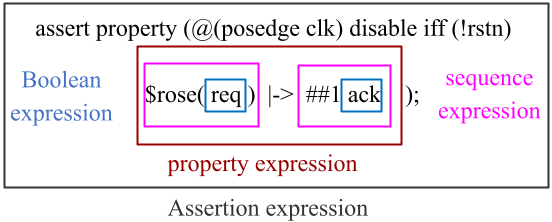
\includegraphics[width=0.52\textwidth]{Figs/FourLayersSVA.png}
  \vspace{8pt}
  \begin{card}
  \small
  A Boolean expression (\texttt{req}) is wrapped by a sequence expression
  (\texttt{\$rose(req) |-> \#\#1 ack}), wrapped by a property expression,
  wrapped by the assertion statement itself -- getting any one layer's
  operator wrong (e.g.\ a sequence operator used where a property operator
  belongs) silently changes the property's meaning rather than raising a
  syntax error.
  \end{card}
\end{frame}

\section{Pipeline Architecture}

\begin{frame}{The original pipeline (MLCAD'25 paper)}
  \framesubtitle{Two stages: HybridRetrieval-Augmented Generation, then SOR}
  \centering
  \resizebox{0.72\textwidth}{!}{%
  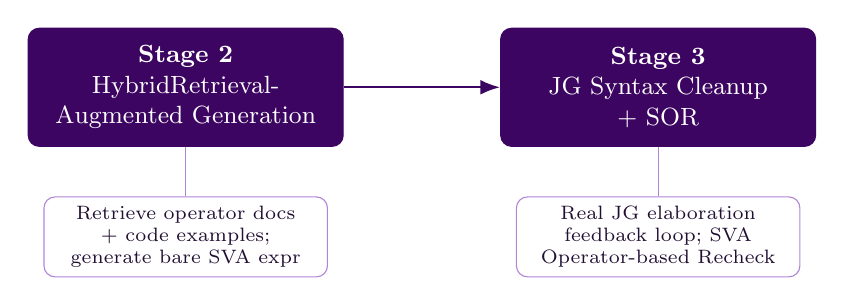
\begin{tikzpicture}[
      stage/.style={rectangle, rounded corners, draw=nyuvioletdark, fill=nyuvioletdark, text=white, minimum width=4cm, minimum height=1.5cm, align=center, font=\small},
      sub/.style={rectangle, rounded corners, draw=nyuvioletlight, fill=white, text=cardtext, minimum width=3.6cm, minimum height=0.9cm, align=center, font=\scriptsize},
      arrow/.style={-{Latex[length=2.5mm]}, thick, nyuvioletdark},
    ]
    \node[stage] (s2) at (0,0) {\textbf{Stage 2}\\HybridRetrieval-\\Augmented Generation};
    \node[stage] (s3) at (6,0) {\textbf{Stage 3}\\JG Syntax Cleanup\\+ SOR};

    \node[sub] (s2a) at (0,-1.9) {Retrieve operator docs\\+ code examples;\\generate bare SVA expr};
    \node[sub] (s3a) at (6,-1.9) {Real JG elaboration\\feedback loop; SVA\\Operator-based Recheck};

    \draw[arrow] (s2) -- (s3);
    \draw[-, nyuvioletlight] (s2) -- (s2a);
    \draw[-, nyuvioletlight] (s3) -- (s3a);
  \end{tikzpicture}}
  \vspace{10pt}
  \begin{card}
  \small
  Given a natural-language property that already names real signals, the
  model retrieves the right operator knowledge, writes a first answer, and
  JasperGold + SOR check and fix it. (Numbered Stage 2/3 to match the
  labels used later in this talk -- Stage 1 is what we added, next slide.)
  \end{card}
\end{frame}

\begin{frame}{As published: the overall pipeline}
  \framesubtitle{The customized RAG framework, from the MLCAD'25 paper}
  \centering
  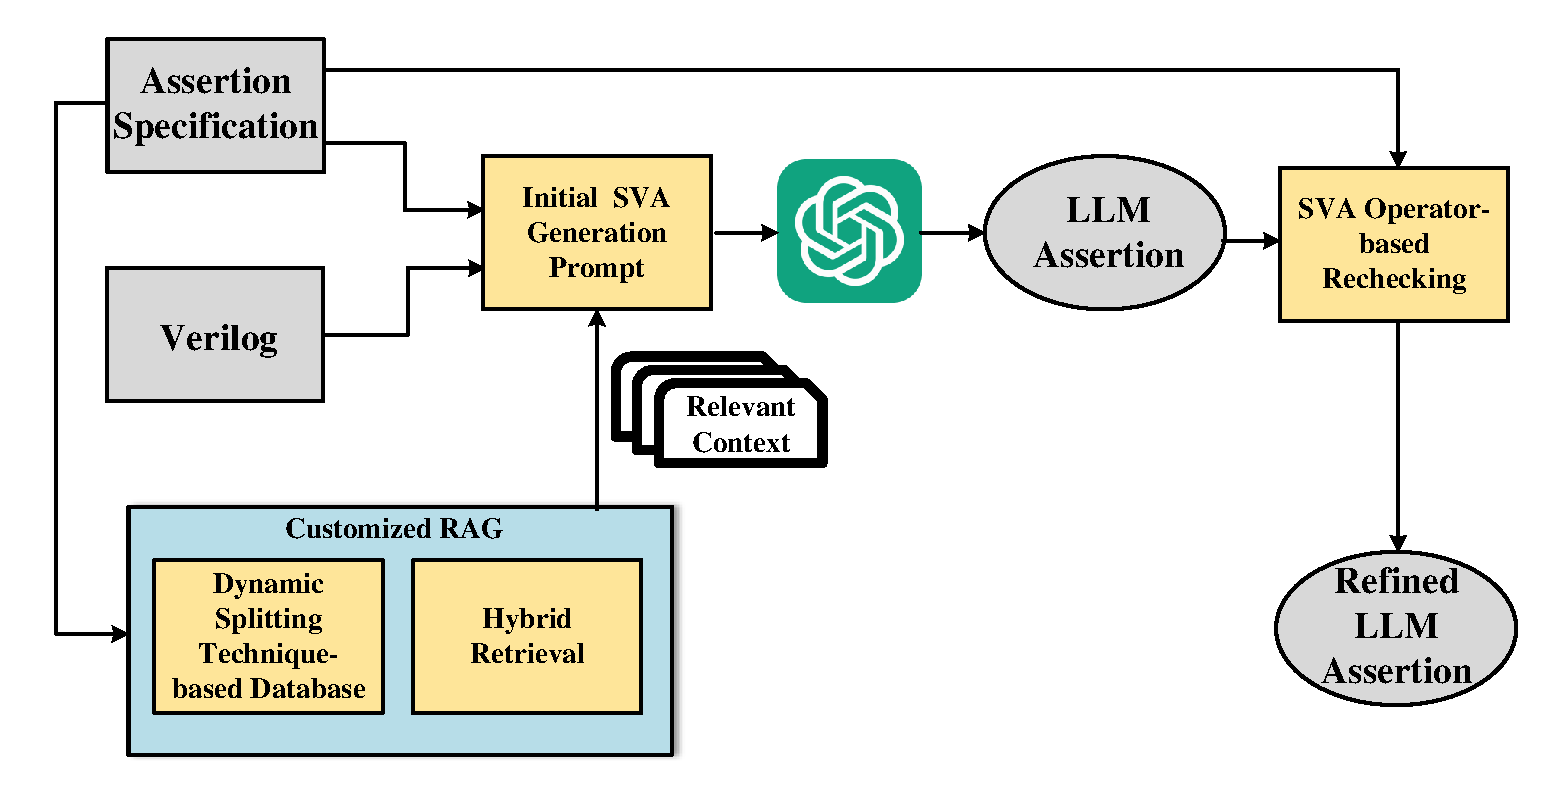
\includegraphics[width=0.62\textwidth]{Figs/RAGSVAG.pdf}
  \vspace{6pt}
  \begin{card}
  \scriptsize
  \textit{Customized RAG} bundles two techniques: \textbf{dynamic
  splitting} (builds a code-centric retrieval database from SVA textbooks,
  preserving each code snippet with its surrounding explanation) and
  \textbf{HybridRetrieval} (next slide). Retrieved context enriches the
  Initial SVA Generation Prompt; the output is then passed through SVA
  Operator-based Rechecking (Stage 3) for a refined final assertion.
  \end{card}
\end{frame}

\begin{frame}{The pipeline today: three stages}
  \framesubtitle{Step 1 (OL-NL grounding) is new -- Stages 2 \& 3 are unchanged from the paper}
  \centering
  \resizebox{\textwidth}{!}{%
  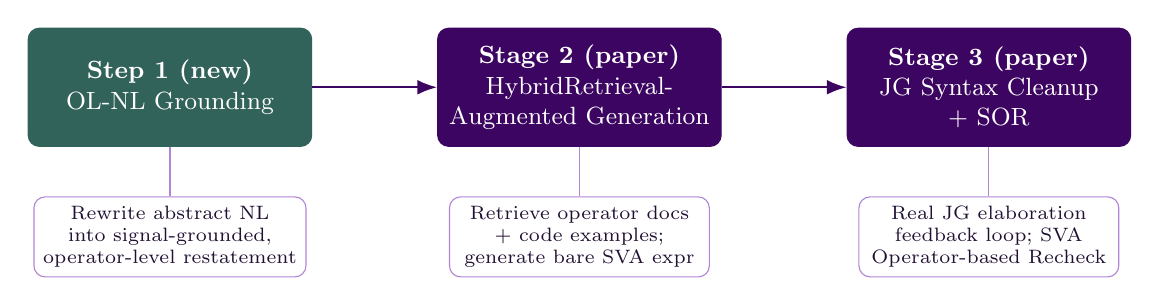
\begin{tikzpicture}[
      stage/.style={rectangle, rounded corners, draw=nyuvioletdark, fill=nyuvioletdark, text=white, minimum width=3.6cm, minimum height=1.5cm, align=center, font=\small},
      newstage/.style={rectangle, rounded corners, draw=goodgreen!70!nyuvioletdark, fill=goodgreen!70!nyuvioletdark, text=white, minimum width=3.6cm, minimum height=1.5cm, align=center, font=\small},
      sub/.style={rectangle, rounded corners, draw=nyuvioletlight, fill=white, text=cardtext, minimum width=3.3cm, minimum height=0.9cm, align=center, font=\scriptsize},
      arrow/.style={-{Latex[length=2.5mm]}, thick, nyuvioletdark},
    ]
    \node[newstage] (s1) at (0,0) {\textbf{Step 1 (new)}\\OL-NL Grounding};
    \node[stage] (s2) at (5.2,0) {\textbf{Stage 2 (paper)}\\HybridRetrieval-\\Augmented Generation};
    \node[stage] (s3) at (10.4,0) {\textbf{Stage 3 (paper)}\\JG Syntax Cleanup\\+ SOR};

    \node[sub] (s1a) at (0,-1.9) {Rewrite abstract NL\\into signal-grounded,\\operator-level restatement};
    \node[sub] (s2a) at (5.2,-1.9) {Retrieve operator docs\\+ code examples;\\generate bare SVA expr};
    \node[sub] (s3a) at (10.4,-1.9) {Real JG elaboration\\feedback loop; SVA\\Operator-based Recheck};

    \draw[arrow] (s1) -- (s2);
    \draw[arrow] (s2) -- (s3);
    \draw[-, nyuvioletlight] (s1) -- (s1a);
    \draw[-, nyuvioletlight] (s2) -- (s2a);
    \draw[-, nyuvioletlight] (s3) -- (s3a);
  \end{tikzpicture}}
  \vspace{10pt}

  \begin{card}
  \small
  Step 1 is only needed when the input isn't already signal-grounded. The
  model is \emph{never} trusted to write the clock/\texttt{disable iff}/label
  itself -- these are added automatically once the bare expression is
  finalized.
  \end{card}
\end{frame}

\begin{frame}[fragile]{Stage 1 in detail: what is OL-NL?}
  \framesubtitle{Only needed when the input doesn't already name real signals}
  \begin{card}
  \scriptsize
  \textbf{OL-NL} = \textbf{operator-level natural language}: a plain-English
  sentence with two rules -- (1) name \emph{only} real signals from the
  design, never a made-up name, and (2) say exactly how those signals
  relate (e.g.\ ``at the same time'' or ``N cycles later''); each such
  relation matches one specific SVA operator, but stays plain words, not
  code.
  \end{card}
  \vspace{3pt}
  \begin{card}
  \tiny
  \textbf{Worked example} (same signals as the earlier SVA):
  \begin{verbatim}
Plain description: that ack correctly follows a request.
  Real signals: req, ack, clk, rstn
OL-NL: Whenever req rises, then exactly 1 clock cycle
later, ack must be asserted.
  \end{verbatim}
  Names only real signals, states the exact timing -- matches
  \texttt{\$rose(req) |-> \#\#1 ack} operator for operator, in plain English.
  \end{card}
  \vspace{3pt}
  \begin{card}
  \tiny
  \textbf{When it runs:} needed when the input doesn't already name real
  signals (\texttt{nl2sva\_human\_verified}); skipped when it already does
  (\texttt{nl2sva\_machine\_verified}). \texttt{--ol-nl-conservative}: stay
  strictly literal -- never add detail the description didn't state.
  \end{card}
\end{frame}

\begin{frame}{Stage 2 in detail: HybridRetrieval-augmented generation}
  \framesubtitle{Two independent retrieval paths feed one generation call -- from the MLCAD'25 paper}
  \centering
  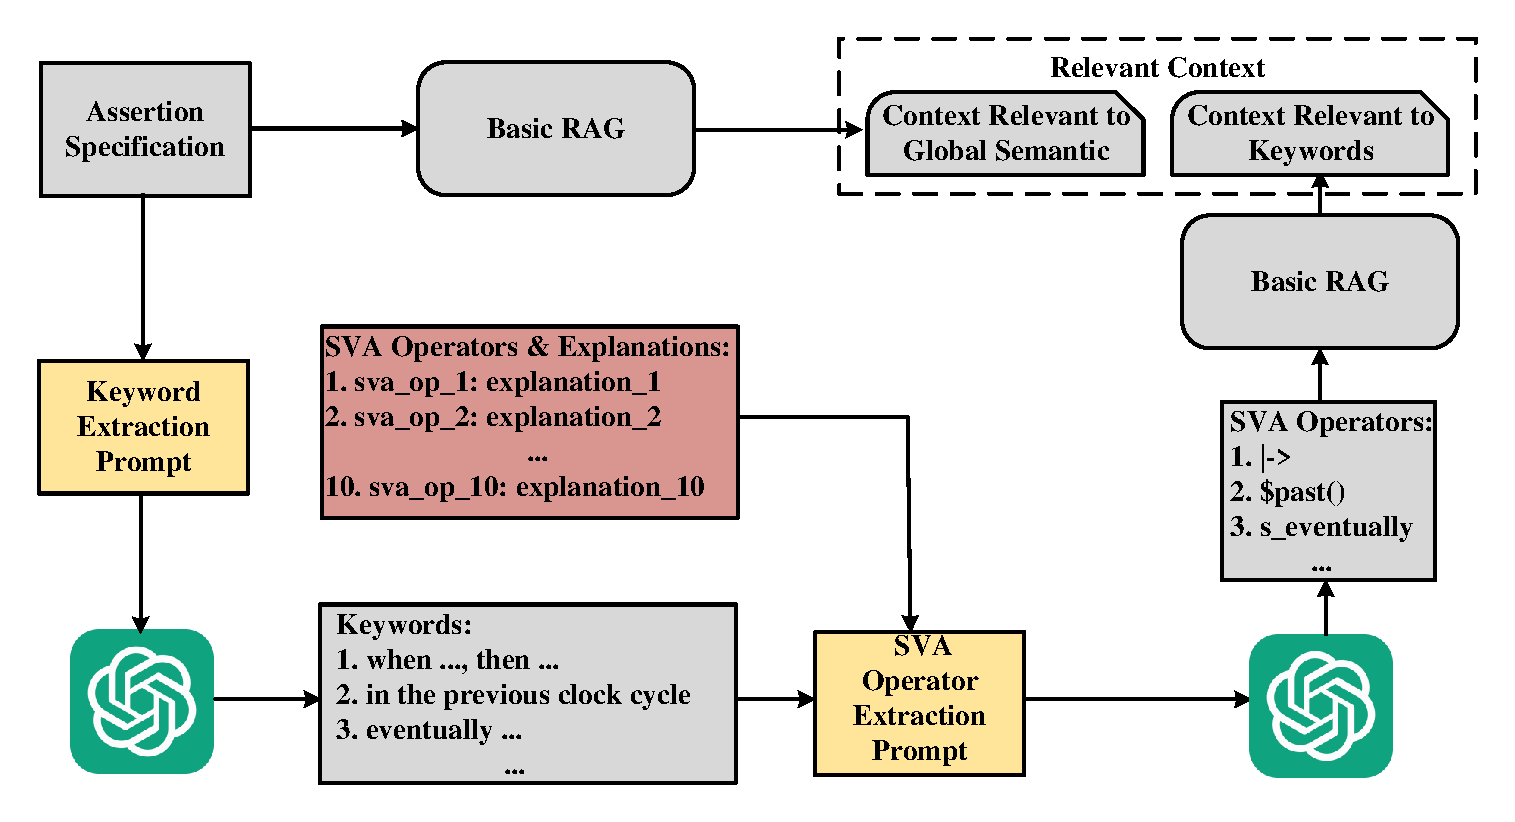
\includegraphics[width=0.58\textwidth]{Figs/HybridRetrieval.pdf}
  \vspace{6pt}
  \begin{card}
  \tiny
  \textbf{Path 1 (top):} Basic RAG on the full assertion specification --
  global-semantic similarity against the code database. \textbf{Path 2
  (bottom):} an LLM decomposes the description into keyword phrases
  (\textit{Keyword Extraction Prompt}), maps each to the closest of 10 SVA
  operators (\textit{SVA Operator Extraction Prompt}), then a second Basic
  RAG pass retrieves chunks specifically discussing those operators. Both
  paths' \textbf{Relevant Context} feeds the single generation call.
  \end{card}
\end{frame}

\begin{frame}{Stage 3 in detail: syntax cleanup + SOR}
  \centering
  \resizebox{0.95\textwidth}{!}{%
  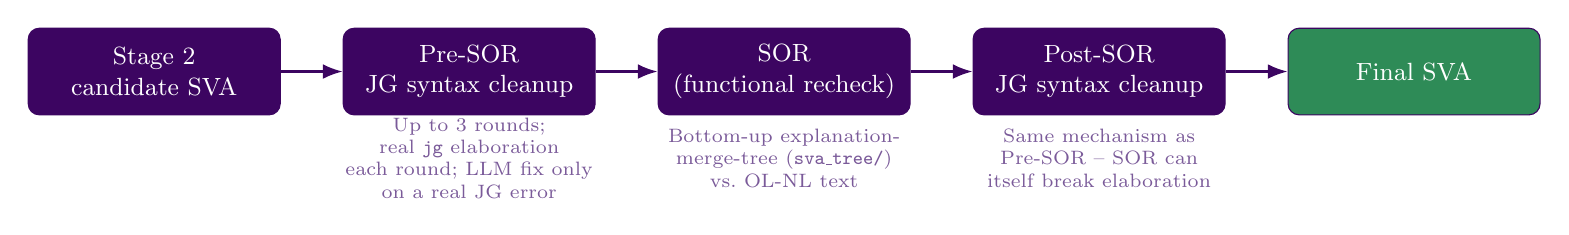
\begin{tikzpicture}[
      node/.style={rectangle, rounded corners, draw=nyuvioletdark, fill=nyuvioletdark, text=white, minimum width=3.2cm, minimum height=1.1cm, align=center, font=\small},
      arrow/.style={-{Latex[length=2.5mm]}, thick, nyuvioletdark},
      note/.style={font=\scriptsize, text=nyumuted, align=center},
    ]
    \node[node] (gen) at (0,0) {Stage 2\\candidate SVA};
    \node[node] (pre) at (4,0) {Pre-SOR\\JG syntax cleanup};
    \node[node] (sor) at (8,0) {SOR\\(functional recheck)};
    \node[node] (post) at (12,0) {Post-SOR\\JG syntax cleanup};
    \node[node, fill=goodgreen] (final) at (16,0) {Final SVA};

    \draw[arrow] (gen) -- (pre);
    \draw[arrow] (pre) -- (sor);
    \draw[arrow] (sor) -- (post);
    \draw[arrow] (post) -- (final);

    \node[note] at (4,-1.1) {Up to 3 rounds;\\real \texttt{jg} elaboration\\each round; LLM fix only\\on a real JG error};
    \node[note] at (8,-1.1) {Bottom-up explanation-\\merge-tree (\texttt{sva\_tree/})\\vs.\ OL-NL text};
    \node[note] at (12,-1.1) {Same mechanism as\\Pre-SOR -- SOR can\\itself break elaboration};
  \end{tikzpicture}}
  \vspace{10pt}
  \begin{card}
  \footnotesize
  \textbf{Confirmed live (Human-69):} SOR combined two implications with an
  invalid \texttt{else} inside a property -- without the post-SOR pass, this
  went straight through as the final answer. Running cleanup \emph{twice}
  (once before, once after SOR) closes that gap.
  \end{card}
\end{frame}

\begin{frame}{As published: SVA operator-based rechecking}
  \framesubtitle{From the MLCAD'25 paper -- the originally published SOR mechanism}
  \centering
  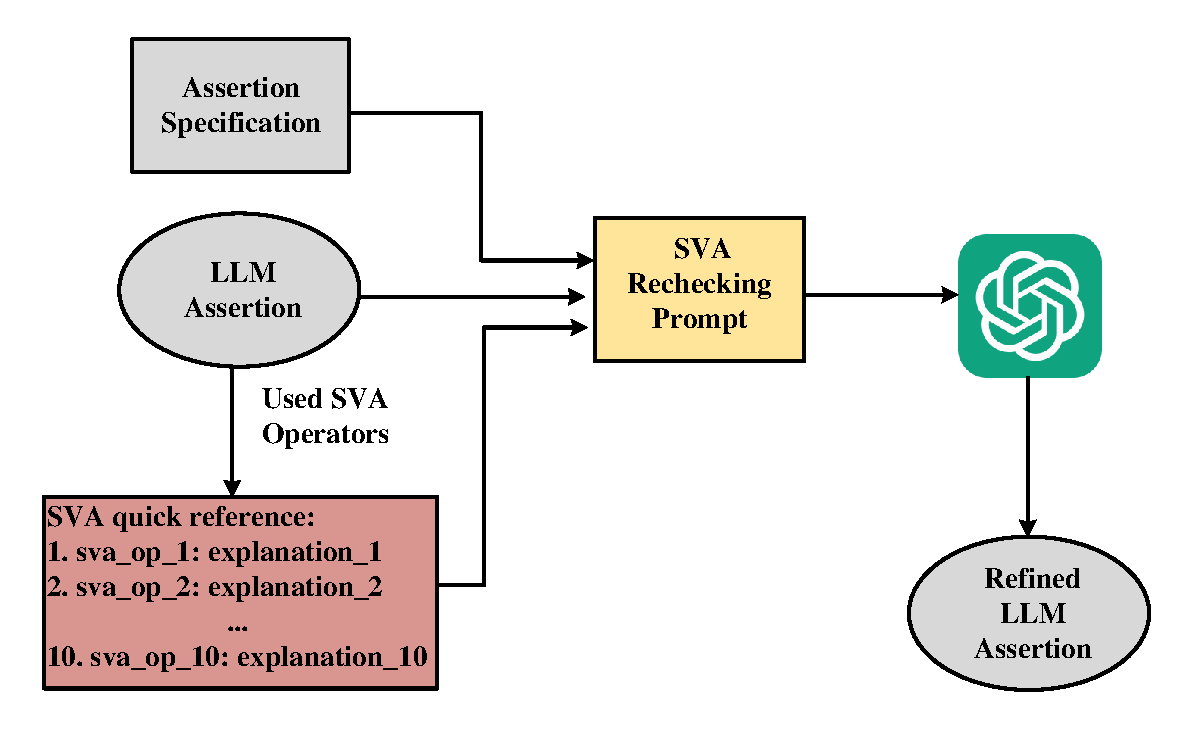
\includegraphics[width=0.5\textwidth]{Figs/SVAOperatorRefine.pdf}
  \vspace{6pt}
  \begin{card}
  \scriptsize
  Extract the operators the LLM assertion actually used, look each one up
  in the SVA quick-reference table, and hand the assertion, the
  specification, and those explanations to a \textit{SVA Rechecking
  Prompt}. \textbf{Since published:} the explanation-merge-tree (next
  slide) replaced this flat operator lookup with a full bottom-up
  rebuild of the assertion's meaning, catching mismatches the
  original per-operator check could miss.
  \end{card}
\end{frame}

\begin{frame}[fragile]{Inside SOR: the explanation-merge-tree}
  \framesubtitle{Parse the candidate's own operator structure bottom-up, then compare}
  \begin{card}
  \scriptsize
  \begin{verbatim}
Candidate SVA:  a && b |-> ##2 c
  \end{verbatim}
  \end{card}
  \vspace{2pt}
  \centering
  \resizebox{0.56\textwidth}{!}{%
  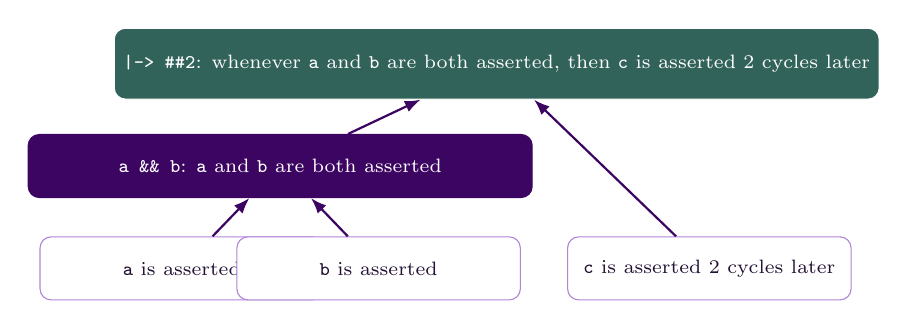
\begin{tikzpicture}[
      leaf/.style={rectangle, rounded corners, draw=nyuvioletlight, fill=white, text=cardtext, minimum width=3.6cm, minimum height=0.8cm, align=center, font=\scriptsize},
      merge/.style={rectangle, rounded corners, draw=nyuvioletdark, fill=nyuvioletdark, text=white, minimum width=6.4cm, minimum height=0.8cm, align=center, font=\scriptsize},
      root/.style={rectangle, rounded corners, draw=white, fill=goodgreen!70!nyuvioletdark, text=white, minimum width=9.5cm, minimum height=0.9cm, align=center, font=\scriptsize},
      arrow/.style={-{Latex[length=2mm]}, thick, nyuvioletdark},
    ]
    \node[leaf] (la) at (-4.0,0) {\texttt{a} is asserted};
    \node[leaf] (lb) at (-1.5,0) {\texttt{b} is asserted};
    \node[leaf] (lc) at (2.7,0) {\texttt{c} is asserted 2 cycles later};

    \node[merge] (mand) at (-2.75,1.3) {\texttt{a \&\& b}: \texttt{a} and \texttt{b} are both asserted};
    \node[root] (root) at (0,2.6) {\texttt{|-> \#\#2}: whenever \texttt{a} and \texttt{b} are both asserted, then \texttt{c} is asserted 2 cycles later};

    \draw[arrow] (la) -- (mand);
    \draw[arrow] (lb) -- (mand);
    \draw[arrow] (mand) -- (root);
    \draw[arrow] (lc) -- (root);
  \end{tikzpicture}}
  \vspace{4pt}
  \begin{card}
  \scriptsize
  \textbf{Compare} the root's composed meaning against the Stage~1 OL-NL
  description. Match $\rightarrow$ confirm verbatim. Mismatch $\rightarrow$
  the model revises -- \texttt{--sor-conservative} tells it to change
  \emph{only} the flagged node (e.g.\ just \texttt{\#\#2}), not rewrite the
  whole property.
  \end{card}
\end{frame}

\section{Key Mechanisms}

\begin{frame}{The bug this talk's improvement targets}
  \framesubtitle{A confirmed, repeated timing error in \texttt{|=>} + \texttt{\#\#N} together}
  \begin{card}
  \scriptsize
  Using \texttt{|=>} (which itself already moves forward one clock cycle)
  together with a written-out \texttt{\#\#N} delay silently lands on \texttt{N+1} total
  cycles instead of \texttt{N} -- both at \textbf{generation time} and
  inside \textbf{SOR's own revision step}, so the error can survive the
  self-correction pass meant to catch it.
  \end{card}
  \vspace{5pt}
  \begin{card}
  \scriptsize
  \textbf{Fix (\texttt{--only-overlap-implication}):} avoid it at the
  root -- always use \texttt{|->}, and always write out any delay with
  \texttt{\#\#N} using the \emph{total} cycle count, instead of combining
  a hidden-cycle operator with a written-out one.
  \end{card}
  \vspace{5pt}
  \begin{card}
  \tiny
  \texttt{--sor-template-timing}: SOR's explanation-merge-tree can also use
  fixed, rule-based, LLM-free templates (\texttt{sva\_temporal\_
  operators.json}'s per-operator fields) instead of an LLM composing each
  node's meaning -- removes another source of the same timing slip.
  \end{card}
\end{frame}

\begin{frame}{The improvement: SOR-timing fixes vs.\ the original pipeline}
  \framesubtitle{Same benchmark rows, same pipeline, only the timing-fix flags differ}
  \begin{card}
  \centering
  \renewcommand{\arraystretch}{1.3}
  \resizebox{\linewidth}{!}{%
  \begin{tabular}{l l r r}
    \toprule
    \textbf{Dataset} & \textbf{Configuration} & \textbf{FM-strict} & \textbf{FM-relaxed} \\
    \midrule
    \multirow{2}{*}{\shortstack[l]{nl2sva\_human\_\\verified (73)}}
      & Original pipeline & 71.2--74.0\% & 83.6--87.7\% \\
      & \textbf{+ SOR-timing fixes} & \textbf{74.0\%} & \textbf{87.7\%} \\
    \midrule
    \multirow{2}{*}{\shortstack[l]{nl2sva\_machine\_\\verified (283)}}
      & Original pipeline & 82.0\% (232/283) & 90.5\% (256/283) \\
      & \textbf{+ SOR-timing fixes} & \textbf{85.2\% (241/283)} & \textbf{95.4\% (270/283)} \\
    \bottomrule
  \end{tabular}}
  \end{card}
  \vspace{8pt}
  \begin{card}
  \scriptsize
  \texttt{sva\_graph.py} also had a real, unrelated parsing bug fixed along
  the way: range/unbounded delays (\texttt{\#\#[M:N]}, \texttt{\#\#[*]},
  \texttt{\#\#[+]}) were mislabeled \texttt{"\#\#None"} internally,
  discarding their real bounds.
  \end{card}
\end{frame}

\section{Evaluation Setup}

\begin{frame}{Benchmark \& metrics}
  \begin{card}
  \textbf{FVEval-Verified} (\href{https://huggingface.co/wyt2000}{wyt2000/FVEval-Verified}):
  a human-expert-corrected version of FVEval's \texttt{nl2sva\_human} and
  \texttt{nl2sva\_machine} benchmarks.
  \begin{itemize}
    \item \textbf{nl2sva\_human\_verified} (73 rows) -- expert-written
      ground-truth SVAs and NL descriptions
    \item \textbf{nl2sva\_machine\_verified} (283 rows) -- rule-generated
      SVAs, LLM-written NL descriptions; bare dummy testbenches, no reset
      signal
  \end{itemize}
  \end{card}
  \vspace{10pt}
  \textbf{Metrics} (all via a real JasperGold \texttt{prop\_eq\_checker}):
  \begin{itemize}
    \item \textbf{SC} (Syntax Correctness) -- does the candidate elaborate
      against the real testbench on its own?
    \item \textbf{FM-strict} -- formally proven full equivalence to the
      golden SVA
    \item \textbf{FM-relaxed} -- FM-strict plus one-directional
      \texttt{implies} matches
  \end{itemize}
\end{frame}

\section{Results: RAG+SOR Pipeline}

\begin{frame}{Cross-model comparison --- RAG+SOR pipeline}
  \framesubtitle{Each row uses that dataset's best-known flag configuration}
  \begin{card}
  \tiny
  \renewcommand{\arraystretch}{1.25}
  \begin{tabular}{l l r r r}
    \toprule
    \textbf{Model} & \textbf{Dataset} & \textbf{SC} & \textbf{FM-strict} & \textbf{FM-relaxed} \\
    \midrule
    gpt-4o & human & 98.6\% (72/73) & 74.0\% (54/73) & 87.7\% (64/73) \\
    gpt-4o & machine & 99.6\% (282/283) & 84.8\% (240/283) & 94.7\% (268/283) \\
    DeepSeek-V4-Flash (thinking) & human & 100.0\% (73/73) & \textbf{86.3\%} (63/73) & \textbf{94.5\%} (69/73) \\
    DeepSeek-V4-Flash (thinking) & machine & 100.0\% (283/283) & \textbf{92.9\%} (263/283) & \textbf{98.6\%} (279/283) \\
    gpt-5 & human & 100.0\% (73/73) & 82.2\% (60/73) & 91.8\% (67/73) \\
    gpt-5 & machine & \statuspill{warnamber}{interrupted (45/283)} & -- & -- \\
    deepseek-chat (thinking off) & human & 100.0\% (73/73) & 74.0\% (54/73) & 80.8\% (59/73) \\
    deepseek-chat (thinking off) & machine & 98.9\% (280/283) & 85.5\% (242/283) & 94.3\% (267/283) \\
    qwen3-8b (Aliyun) & human & 91.8\% (67/73) & 35.6\% (26/73) & 53.4\% (39/73) \\
    qwen3-8b (Aliyun) & machine & 88.7\% (251/283) & 60.8\% (172/283) & 73.9\% (209/283) \\
    qwen3-14b (Aliyun) & human & 91.8\% (67/73) & 65.8\% (48/73) & 79.5\% (58/73) \\
    qwen3-14b (Aliyun) & machine & 95.1\% (269/283) & 81.6\% (231/283) & 90.8\% (257/283) \\
    \bottomrule
  \end{tabular}
  \end{card}
  \vspace{4pt}
  {\scriptsize\textcolor{nyumuted}{DeepSeek-V4-Flash (thinking) was originally run and labeled ``DeepSeek-R1''
  -- DeepSeek has since silently remapped the \texttt{deepseek-reasoner} API
  alias to route to V4-Flash with thinking mode on; relabeled accordingly.}}
\end{frame}

\begin{frame}{Cross-model comparison --- raw model output (no pipeline)}
  \framesubtitle{Same JasperGold scorer, no RAG / OL-NL grounding / SOR}
  \begin{card}
  \tiny
  \renewcommand{\arraystretch}{1.25}
  \begin{tabular}{l l r r r}
    \toprule
    \textbf{Model} & \textbf{Dataset} & \textbf{SC} & \textbf{FM-strict} & \textbf{FM-relaxed} \\
    \midrule
    gpt-4o (0-shot) & human & 94.5\% (69/73) & 63.0\% (46/73) & 76.7\% (56/73) \\
    CodeV-SVA-8B & human & 97.3\% (71/73) & 75.3\% (55/73) & 83.6\% (61/73) \\
    CodeV-SVA-14B & human & 93.2\% (68/73) & 74.0\% (54/73) & 80.8\% (59/73) \\
    CodeV-SVA-8B & machine & 96.5\% (273/283) & 83.0\% (235/283) & 93.3\% (264/283) \\
    CodeV-SVA-14B & machine & 97.2\% (275/283) & 80.9\% (229/283) & 93.3\% (264/283) \\
    DeepSeek-V4-Flash (thinking, 0-shot) & human & 98.6\% (72/73) & 76.7\% (56/73) & 93.2\% (68/73) \\
    DeepSeek-V4-Flash (thinking, 0-shot) & machine & 100.0\% (283/283) & 90.8\% (257/283) & 98.2\% (278/283) \\
    deepseek-chat (thinking off, 0-shot) & human & 94.5\% (69/73) & 54.8\% (40/73) & 76.7\% (56/73) \\
    deepseek-chat (thinking off, 0-shot) & machine & 97.5\% (276/283) & 78.4\% (222/283) & 89.4\% (253/283) \\
    qwen3-8b (Aliyun, base) & human & 89.0\% (65/73) & 35.6\% (26/73) & 57.5\% (42/73) \\
    qwen3-8b (Aliyun, base) & machine & 87.6\% (248/283) & 51.2\% (145/283) & 66.8\% (189/283) \\
    qwen3-14b (Aliyun, base) & human & 93.2\% (68/73) & 49.3\% (36/73) & 69.9\% (51/73) \\
    qwen3-14b (Aliyun, base) & machine & 91.9\% (260/283) & 65.7\% (186/283) & 76.3\% (216/283) \\
    \bottomrule
  \end{tabular}
  \end{card}
  \vspace{4pt}
  \scriptsize\textbf{Takeaway:} the pipeline (RAG + OL-NL grounding + SOR) lifts gpt-4o's
  FM-strict from 63.0\%$\to$74.0\% (human) and (with the machine config) from
  a similarly weak 0-shot baseline to 84.8\% -- a real, structural gain
  from retrieval + self-correction, not just a stronger base model.
\end{frame}

\begin{frame}{Case study: when the pipeline does \emph{not} help}
  \framesubtitle{qwen3-8b on nl2sva\_human\_verified}
  \begin{columns}[T]
    \begin{column}{0.55\textwidth}
      \begin{card}
      \footnotesize
      \textbf{Net effect: no real change.}
      \begin{itemize}
        \item FM-strict identical: 26/73 both ways
        \item FM-relaxed \emph{slightly worse}: 53.4\% vs.\ 57.5\%
        \item 12/73 rows flip fail$\to$pass \dots
        \item \dots but a near-equal 12/73 flip pass$\to$fail
      \end{itemize}
      \end{card}
    \end{column}
    \begin{column}{0.45\textwidth}
      \textbf{Three ways it got worse:}
      \begin{itemize}
        \item An extra, unneeded \texttt{\#\#N} added where none was needed
        \item A boolean's polarity flipped while ``fixing'' something else
        \item A correct plain comparison rewritten into a non-equivalent
          \texttt{\$onehot0(\{...\})} form
      \end{itemize}
    \end{column}
  \end{columns}
  \vspace{10pt}
  \begin{card}
  \small
  \textbf{Conclusion:} the pipeline's net benefit scales with the base
  model's own ability to self-correct \emph{without introducing new errors}
  during revision -- not something that is true for every model, no matter
  what. (nl2sva\_machine\_verified does \emph{not} show this no-change
  pattern for the same model: 60.8\% vs.\ 51.2\% FM-strict.)
  \end{card}
\end{frame}

% ============================================================================
\dividerframe{II}{End-to-End Spec2SVA}

\section{Motivation}

\begin{frame}{From ready-made benchmarks to real designs}
  \begin{columns}[T]
    \begin{column}{0.5\textwidth}
      \textbf{What Part I evaluated:} \\
      NL2SVA on FVEval-Verified -- properties and RTL are already picked
      out and ready to use, one property per row, always paired with a
      golden (known-correct) SVA.
    \end{column}
    \begin{column}{0.5\textwidth}
      \textbf{What real verification looks like:} \\
      a \emph{specification document} (PDF, dozens of pages) and a
      \emph{multi-file RTL design} -- no pre-extracted property list, no
      golden SVA to check against.
    \end{column}
  \end{columns}
  \vspace{10pt}
  \begin{card}
    \textbf{Goal:} close the loop -- \emph{Spec2NL} (turn a spec + RTL into a
    list of natural-language verification properties) feeding directly into
    \emph{our} NL2SVA pipeline, with JasperGold verifying the result end to
    end.
  \end{card}
\end{frame}

\section{AssertionForge: Spec2NL}

\begin{frame}{AssertionForge (NVlabs, LAD 2025)}
  \framesubtitle{\href{https://github.com/NVlabs/AssertionForge}{github.com/NVlabs/AssertionForge} --- \href{https://arxiv.org/abs/2503.19174}{arXiv:2503.19174}}
  \begin{itemize}
    \item \textbf{Stage 1 -- Knowledge Graph Construction:} builds a joint
      KG from the spec (via GraphRAG, domain-customized entity-extraction
      prompt) and the RTL (\texttt{pyverilog}-based structural analysis),
      then fuses the two
    \item \textbf{Stage 2 -- Test Plan Generation:} for each architectural
      signal, retrieves KG-guided context (RAG chunks + graph-path
      analysis), prunes with an LLM judge, and generates natural-language
      verification \emph{plans}
  \end{itemize}
  \vspace{8pt}
  \begin{card}
  \footnotesize
  Stage 1 + Stage 2 together $=$ \textbf{Spec2NL}: spec PDF + RTL directory
  $\rightarrow$ a list of natural-language properties, each grounded in a
  specific signal and its role in the design.
  \end{card}
\end{frame}

\section{Integration Architecture}

\begin{frame}{Spec2NL + NL2SVA = end-to-end Spec2SVA}
  \centering
  \vspace{6pt}
  \resizebox{0.88\textwidth}{!}{%
  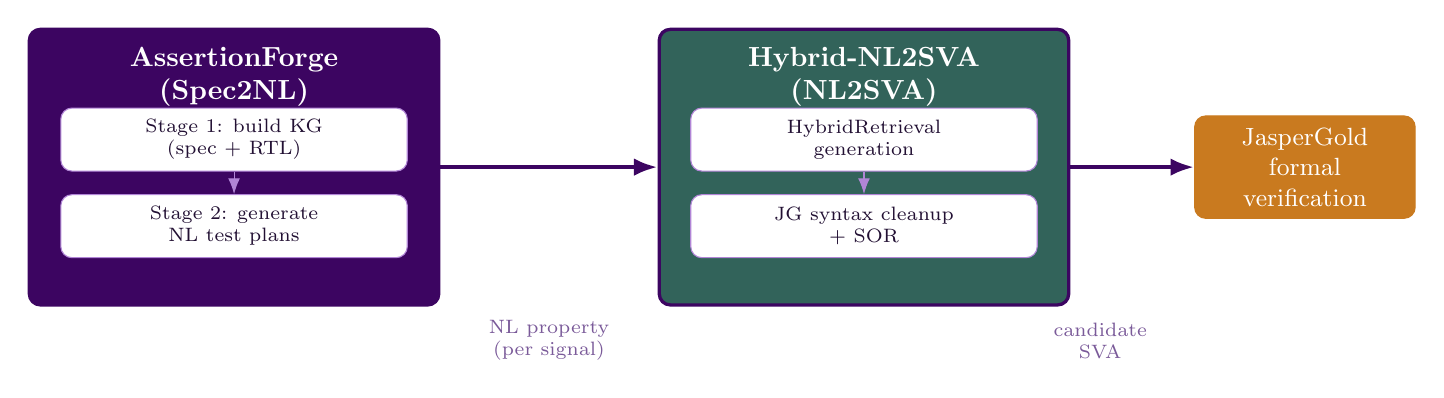
\begin{tikzpicture}[
      big/.style={rectangle, rounded corners, draw=nyuvioletdark, very thick, minimum width=5.2cm, minimum height=2.9cm, align=center},
      inner/.style={rectangle, rounded corners, draw=nyuvioletlight, fill=white, text=cardtext, minimum width=4.4cm, minimum height=0.8cm, align=center, font=\scriptsize},
      arrow/.style={-{Latex[length=3mm]}, ultra thick, nyuvioletdark},
    ]
    \node[big, minimum height=3.5cm, fill=nyuvioletdark] (af) at (0,0) {};
    \node[align=center, text=white, font=\bfseries] at (0,1.15) {AssertionForge\\(Spec2NL)};
    \node[inner] (af1) at (0,0.35) {Stage 1: build KG\\(spec + RTL)};
    \node[inner] (af2) at (0,-0.75) {Stage 2: generate\\NL test plans};
    \draw[-{Latex[length=2mm]}, nyuvioletlight] (af1) -- (af2);

    \node[big, minimum height=3.5cm, fill=goodgreen!70!nyuvioletdark] (hn) at (8,0) {};
    \node[align=center, text=white, font=\bfseries] at (8,1.15) {Hybrid-NL2SVA\\(NL2SVA)};
    \node[inner] (hn1) at (8,0.35) {HybridRetrieval\\generation};
    \node[inner] (hn2) at (8,-0.75) {JG syntax cleanup\\+ SOR};
    \draw[-{Latex[length=2mm]}, nyuvioletlight] (hn1) -- (hn2);

    \node[rectangle, rounded corners, draw=warnamber, fill=warnamber, text=white, minimum width=2.8cm, minimum height=1.3cm, align=center, font=\small] (jg) at (13.6,0) {JasperGold\\formal\\verification};

    \draw[arrow] (af) -- (hn);
    \draw[arrow] (hn) -- (jg);

    \node[font=\scriptsize, text=nyumuted, align=center] at (4,-2.2) {NL property\\(per signal)};
    \node[font=\scriptsize, text=nyumuted, align=center] at (11,-2.2) {candidate\\SVA};
  \end{tikzpicture}}
  \vspace{10pt}
  \begin{card}
    \footnotesize
    NL2SVA runs with \textbf{the same flag configuration as the
    nl2sva\_machine\_verified evaluation}: \texttt{--skip-signal-list-note
    --sor-conservative --only-overlap-implication}, no \texttt{--ol-nl-grounding}
    (AssertionForge's plans are already signal-grounded) --- plus a new
    \texttt{clock\_signal} parameter (real RTL rarely names its clock
    \texttt{clk}).
  \end{card}
\end{frame}

\section{UART Pilot}

\begin{frame}{Case study: UART}
  \framesubtitle{\href{https://github.com/hkust-zhiyao/AssertLLM}{AssertLLM}'s spec + RTL}
  \begin{columns}[T]
    \begin{column}{0.48\textwidth}
      \textbf{Design.}
      \begin{itemize}
        \item 6 Verilog modules: \texttt{uart2bus\_top} (real top),
          \texttt{uart\_top}, \texttt{baud\_gen}, \texttt{uart\_rx},
          \texttt{uart\_tx}, \texttt{uart\_parser}
        \item 246 total signals; 18 architectural (interface) signals
          across the hierarchy
        \item Real clock port name: \texttt{clock} (not \texttt{clk})
      \end{itemize}
    \end{column}
    \begin{column}{0.48\textwidth}
      \textbf{Spec2NL output.}
      \begin{itemize}
        \item Knowledge graph: 1{,}371 nodes, 1{,}620 edges (spec $+$ RTL fused)
        \item \textbf{323} natural-language verification properties
          generated (all 18 signals)
        \item QiMeng-CodeV-SVA's own Table~5 reports \textbf{265} SVAs for
          UART (GPT-4o Spec2NL + GPT-4o NL2SVA) -- same order of magnitude
      \end{itemize}
    \end{column}
  \end{columns}
  \vspace{6pt}
  \begin{card}
    \scriptsize
    \textbf{A real gap found \& fixed along the way:} upstream's
    \texttt{valid\_signals} example only listed 2 of 18 signals; and
    \texttt{utils\_LLM.py}/\texttt{utils\_LLM\_client.py} ship as empty ``add
    your own client'' stubs -- both needed fixing before Stage 1/2 ran end to end.
  \end{card}
\end{frame}

\begin{frame}[fragile]{Sample generated NL properties}
  \begin{card}
  \scriptsize
  \begin{itemize}
    \item \textbf{baud\_clk:} ``that after a reset condition, baud\_clk will
      resume toggling without skipping cycles based on the previously set
      value of baud\_freq''
    \item \textbf{baud\_freq:} ``that baud\_freq maintains a constant value
      when the \texttt{global\_clock\_freq} and \texttt{baud\_rate} inputs
      remain unchanged over 20 clock cycles''
    \item \textbf{int\_req / int\_gnt:} bus request/grant handshake
      properties derived from path analysis between \texttt{uart2bus\_top}'s
      internal bus interface signals
  \end{itemize}
  \end{card}
  \vspace{10pt}
  \begin{card}
  \footnotesize
  Example NL2SVA output (\texttt{clock\_signal=clock}, no \texttt{disable iff},
  matching the machine-dataset config):
  \begin{verbatim}
asrt: assert property (@(posedge clock)
    (new_tx_data && !tx_busy) |-> tx_data
);
  \end{verbatim}
  \end{card}
\end{frame}

\section{Results}

\begin{frame}{UART: full NL2SVA + formal verification results}
  \framesubtitle{323-property run via Hybrid-NL2SVA (gpt-4o, machine config), scored with JasperGold}
  \begin{card}
  \centering
  \renewcommand{\arraystretch}{1.3}
  \resizebox{\linewidth}{!}{%
  \begin{tabular}{l r r r}
    \toprule
    \textbf{Spec2NL / NL2SVA} & \textbf{\#SVA} & \textbf{\#SynC} & \textbf{\#Proven} \\
    \midrule
    QiMeng-CodeV-SVA: GPT-4o / GPT-4o & 265 & 186 (70.2\%) & 54 (20.4\%) \\
    Ours -- all 18 signals & 323 & 225 (69.7\%) & 60 (18.6\%) \\
    \bottomrule
  \end{tabular}}
  \end{card}
  \vspace{10pt}
  \begin{card}
    \footnotesize
    \textbf{Caveat:} we independently reconstructed the 18-signal
    \texttt{valid\_signals} list (the cloned config only had a 2-signal
    placeholder); we have no evidence the paper's own run used the same
    signal scope, so this is not a strict apples-to-apples comparison --
    only evidence our pipeline lands in a reasonable, self-consistent range.
    \#Proven checked via a new \texttt{check\_sva\_proven} utility
    (\texttt{prove -all} + \texttt{get\_status}, no golden SVA needed).
  \end{card}
\end{frame}

\begin{frame}{A methodology gap: properties about free inputs}
  \framesubtitle{AssertionForge's own few-shot prompt (\texttt{get\_sva\_icl\_examples}) is entirely PWDATA-shaped}
  \begin{card}
  \scriptsize
  \textit{``that the input data PWDATA has a value between 83 and 165 \dots\ 3 clock
  cycles after reset deasserted''} -- \texttt{PWDATA} is APB's free bus-input
  signal; every one of AssertionForge's 5 hardcoded style examples follows
  this same shape.
  \end{card}
  \vspace{8pt}
  \begin{card}
  \centering
  \renewcommand{\arraystretch}{1.3}
  \resizebox{\linewidth}{!}{%
  \begin{tabular}{l r r}
    \toprule
    \textbf{UART signal subset} & \textbf{n} & \textbf{\#Proven} \\
    \midrule
    Free inputs / out-of-scope (\texttt{ser\_in}, \texttt{int\_rd\_data}, \texttt{int\_gnt}, \texttt{ce\_16}) & 67 & 11.9\% \\
    \textbf{Design-controlled only} (outputs + internal wires) & \textbf{256} & \textbf{20.3\%} \\
    \bottomrule
  \end{tabular}}
  \end{card}
  \vspace{4pt}
  \begin{card}
    \tiny
    A primary \emph{input} port is free/unconstrained under JasperGold with
    no environment \texttt{assume}s -- a property claiming ``this input
    settles into range X'' is nearly impossible to prove, just because of
    how the design is built, regardless of NL2SVA quality. Excluding these 4 signals lifts \#Proven
    from 18.6\%$\to$\textbf{20.3\%}, matching the GPT-4o/GPT-4o reference
    almost exactly. (\texttt{ce\_16}: declared inside \texttt{uart\_top}, one
    level below our assertion scope \texttt{uart2bus\_top} -- not even a
    valid identifier there.)
  \end{card}
\end{frame}

\begin{frame}{A second gap: signal hallucination, not just free inputs}
  \framesubtitle{Of 98 syntax-fail rows, ``X' is not declared'' errors name 68 distinct identifiers}
  \begin{card}
  \centering
  \renewcommand{\arraystretch}{1.3}
  \resizebox{\linewidth}{!}{%
  \begin{tabular}{l r}
    \toprule
    \textbf{Category (checked against the 6 real RTL files)} & \textbf{occurrences} \\
    \midrule
    Real RTL identifiers used at the \emph{wrong scope} (e.g.\ \texttt{ce\_16}$\times$34, \texttt{bit\_count}$\times$26, \texttt{ce\_1}$\times$22) & 21 distinct \\
    Pure hallucinations, not found anywhere in the RTL (\texttt{local\_global\_clock\_freq}, \texttt{logic\_counter}, \dots) & 47 distinct \\
    \bottomrule
  \end{tabular}}
  \end{card}
  \vspace{8pt}
  \begin{card}
    \footnotesize
    \textbf{But most of this traces back further, to the NL plans
    themselves:} of 338 undeclared-identifier occurrences, \textbf{236
    (69.8\%)} have their ``core'' name \emph{literally present in the
    corresponding NL plan's own text} -- e.g.\ the \texttt{baud\_freq} plan on
    the earlier slide reads \textit{``\dots\ using the formula
    16*baud\_rate / gcd(global\_clock\_freq, 16*baud\_rate)''}, and NL2SVA
    just copied \texttt{baud\_rate}/\texttt{global\_clock\_freq} word for word
    as identifiers -- except neither is a real RTL signal. This is a
    Spec2NL grounding gap, not (only) an NL2SVA one.
  \end{card}
\end{frame}

\begin{frame}[fragile]{Root cause: real RTL documentation, not noise}
  \framesubtitle{\texttt{baud\_gen.v}'s own header comment, verbatim}
  \begin{card}
  \scriptsize
  \begin{verbatim}
// the two registers should be calculated as follows:
//   baud_freq  = 16*baud_rate / gcd(global_clock_freq, 16*baud_rate)
//   baud_limit = (global_clock_freq / gcd(...)) - baud_freq
  \end{verbatim}
  \end{card}
  \vspace{5pt}
  \begin{card}
    \scriptsize
    \texttt{baud\_freq} is an \emph{input} to \texttt{baud\_gen} --
    \texttt{baud\_rate}/\texttt{global\_clock\_freq} never appear as actual
    Verilog identifiers anywhere in the 6 files, only in this comment. True,
    directly-relevant content, not retrieval noise -- the model has good
    reason to want to cite it.
  \end{card}
  \vspace{4pt}
  \begin{card}
    \scriptsize
    \textbf{Prompt-only fixes made this WORSE, not better}, across several
    revisions -- we saw the same pattern elsewhere too: naming the exact
    bad thing to avoid puts it right in front of the model, and it tends
    to copy it instead of avoiding it. Invalid-signal leakage rose
    14\%$\to$22\%$\to$27\%$\to$30\% across several tries, one after
    another, to ban it in words.
  \end{card}
\end{frame}

\begin{frame}{Fix: two-step generation + a mechanical filter}
  \framesubtitle{Reworking AssertionForge's Stage 2 (\texttt{gen\_plan.py}) directly}
  \begin{card}
  \scriptsize
  \begin{itemize}
    \item \textbf{Step 1 (idea):} free-form property ideas, no precision
      rules at all -- just ``what's worth testing''
    \item \textbf{Step 2 (OL-NL grounding):} rewrites Step 1's ideas into
      precise, signal-grounded form -- valid-signal whitelist,
      operator-level/sequential-vs-combinational discipline, vague-qualifier
      / trailing-rationale / gcd bans, the \emph{same} SVA Operator Context
      table Hybrid-NL2SVA's own Stage 1 uses -- literally the same grounding
      task Stage 1 performs, on AssertionForge's side instead
    \item \textbf{Mechanical filter (post-hoc, not a prompt):} drops any
      grounded plan still referencing a snake\_case, signal-shaped token not
      in \texttt{valid\_signals} -- carries none of the copy-the-bad-example
      risk above, since it never goes back into a prompt
  \end{itemize}
  \end{card}
  \vspace{8pt}
  \begin{card}
    \footnotesize
    \textbf{Lesson:} banning a specific bad pattern \emph{in words} tends
    to make it worse; moving the same rule \emph{out of the prompt} into a
    mechanical check is what actually worked.
  \end{card}
\end{frame}

\begin{frame}{Validated: same 44 properties, ungrounded vs.\ grounded}
  \framesubtitle{\texttt{baud\_clk}/\texttt{baud\_freq} pilot -- the exact same starting ideas, matched one to one}
  \begin{card}
  \centering
  \renewcommand{\arraystretch}{1.3}
  \resizebox{\linewidth}{!}{%
  \begin{tabular}{l r r r}
    \toprule
    \textbf{Same 44 properties, different generation} & \textbf{n} & \textbf{\#SynC} & \textbf{\#Proven} \\
    \midrule
    Raw ideas + gpt-4o 0-shot baseline (no pipeline) & 44 & 30 (68.2\%) & 15 (34.1\%) \\
    Raw ideas + CodeV-SVA-8B (no pipeline) & 44 & 18 (40.9\%) & 12 (27.3\%) \\
    Raw ideas + CodeV-SVA-14B (no pipeline) & 44 & 21 (47.7\%) & 13 (29.5\%) \\
    \textbf{Grounded (Step 2 + filter) + full Hybrid-NL2SVA} & \textbf{44} & \textbf{40 (90.9\%)} & \textbf{24 (54.5\%)} \\
    \bottomrule
  \end{tabular}}
  \end{card}
  \vspace{5pt}
  \begin{card}
    \scriptsize
    Same 44 properties both ways (matched one to one) -- grounding + the
    full pipeline is \textbf{+22.7pp \#SynC, +20.4pp \#Proven} over the best
    ungrounded baseline; a specialized NL2SVA model alone (CodeV-SVA)
    can't make up for bad, made-up signal names the way grounding
    does. \textit{Scope: \texttt{baud\_clk}/\texttt{baud\_freq} only (2/18
    signals) -- a small test before the remaining 16 signals and a full
    re-run.}
  \end{card}
\end{frame}

\section{Next Steps}

\begin{frame}{Next steps}
  \begin{itemize}
    \item Run the two-step generation + mechanical filter on the remaining
      16 signals and fully regenerate \texttt{nl\_plans\_uart.txt}
    \item Extend the pilot to the remaining 4 designs from QiMeng-CodeV-SVA's
      Table~5 (APB, ETHMAC, OPENMSP430, SOCKIT)
    \item Swap AssertionForge's own NL2SVA backend for a head-to-head
      comparison at the \emph{same} Spec2NL properties
    \item Try DeepSeek-V4-Flash / qwen3 as AssertionForge's own
      Spec2NL backend, not just gpt-4o
    \item Look into why \#SynC (69.7\%) trails \#SVA -- categorize the
      elaboration failures the same way Part I's row-by-row diffing did
  \end{itemize}
  \vspace{16pt}
  \begin{center}
    \Large\textbf{Thank you}
  \end{center}
\end{frame}

\end{document}
